\scanpage{82}
de la catégorie de ces modules vers $C$ est pleinement fidèle, et son image essentielle est formée des objets $X'$ de $C$ qui sont localement sur $S$ isomorphes à un objet de la forme $X^n$.

NB\quad La conclusion de b) est satisfaite si, au lieu de supposer $C$ localisable, on la suppose stable par facteurs directs (=karoubienne), et \deleted{en fait $P$} si on prend des $P$ projectifs de type fini sur $R$.

c)\quad Soit toujours $R$ une $A$-algèbre\unsure{ \inserted{de type fini},|, \inserted{de type fini}} et soit $\operatorname{Mod}\unsure{\deleted{f}(|(}R,C)$ la catégorie des objets de $R$ munis d'une opération $R$-linéaire. \unsure{\deleted{C}A|\deleted{A}C}'est une catégorie $A$-li\unsure{néé|né}aire, et \unsure{\deleted{d}l|\deleted{l}d}a catégorie fibrée des
\figure{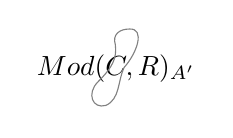
\begin{tikzpicture}[baseline=(m.base)]
\node (m) at (0,0) {$\operatorname{Mod}(\uuline{C},R)_{A'}$};
\handwritten{\draw[gray] (.17,.50) .. controls (.37,.51) and (.27,.20) .. (.10,.01) .. controls (.02,-.16) and (.05,-.39) .. (-.13,-.47) .. controls (-.30,-.52) and (-.38,-.32) .. (-.23,-.17) .. controls (-.04,.02) and (.01,.13) .. (-.01,.30) .. controls (-.05,.43) and (.04,.50) .. (.17,.50);}
\end{tikzpicture}}
(pour $A'$ \deleted{anneau} \deleted{affine d'un ouvert affine de $S=\operatorname{Spec}(A)$)}\inserted{une $A$-algèbre)} est équivalente à la catégorie fibrée des sections de $\uline{C}$ munis d'une opération de $R$\unsure{\deleted{n}.|n} \unsure{En|Bn} particulier, sa restriction au \deleted{site} petit site zariskien affine de $S$ \deleted{\unsure{site|sitd}} s'identifie à
\figure{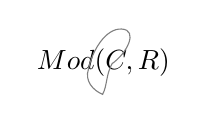
\begin{tikzpicture}[baseline=(m.base)]
\node (m) at (0,0) {$\operatorname{Mod}(\uline{C},R)$};
\handwritten{\draw[gray] (.23,.43) .. controls (.45,.42) and (.30,.12) .. (.11,-.01) .. controls (.03,-.16) and (.05,-.29) .. (-.01,-.40) .. controls (-.13,-.35) and (-.24,-.23) .. (-.19,-.08) .. controls (-.14,.16) and (.03,.44) .. (.23,.43);}
\end{tikzpicture}}
; c'est donc un champ si $\uline{C}$ en est un, donc $\operatorname{Mod}(R,\unsure{\deleted{C}|\mathbb{C}|\mathbb{A}})$ est localisable \inserted{s\unsure{\deleted{e}u|\deleted{u}e}r $S$} si $C$ l'est.

NB\quad Si $R$ est commutatif, $\operatorname{Mod}(R,C)$ est même $R$-linéaire. Notre raisonnement \uline{ne prouve pas} que \deleted{$C$ est} $\operatorname{Mod}(R,C)$ est local\deleted{\unsure{r|i}}isable sur $R$ i.e. sur $\operatorname{Spec}(R)$ (ce qui est plus fort que de dire qu'elle est localisable sur $S=\operatorname{Spec}(A)$).

d)\quad \deleted{Deux objets de $\unsure{X',Y|X;Y}$ de $C$ tels que sont dits} Si $C$ est localisable sur $A$, alors pour $A'$ \deleted{ouvert} anneau affine d'un ouvert affine \inserted{$U$} de $S$, $C_{A'}$ est localisable sur $A'$, et le champ associé sur $U$ s'identifie à la restriction d\unsure{\deleted{e}u|\deleted{u}e} champ $\uline{C}$ à $U$.

e)\quad Deux objets de $C$ sont dits apparentés (ou $A$-\unsure{\deleted{p}a|\deleted{a}p}pparentés) s'ils sont localement isomorphes sur $A$. \unsure{\deleted{D}C|\deleted{C}D}'est évidemment une relation d'équivalence, et la sous-catégorie pleine de $C$ formée des objets apparentés à un objet de $C$ est une catégorie \deleted{de} $A$-linéaire localisable sur $A$, et c'est une catégorie de Deuring,
% archive sheet number: 81
